%%%%%%%%%%%%%%%%%%%%%%%%%%%%%%%%%%%%
% Slide options
%%%%%%%%%%%%%%%%%%%%%%%%%%%%%%%%%%%%

% Option 1: Slides with solutions

\documentclass[slidestop,compress,mathserif]{beamer}
\newcommand{\soln}[1]{\textit{#1}}
\newcommand{\solnGr}[1]{#1}

% Option 2: Handouts without solutions

%\documentclass[11pt,containsverbatim,handout]{beamer}
%\usepackage{pgfpages}
%\pgfpagesuselayout{4 on 1}[letterpaper,landscape,border shrink=5mm]
%\newcommand{\soln}[1]{ }
%\newcommand{\solnGr}{ }

%%%%%%%%%%%%%%%%%%%%%%%%%%%%%%%%%%%%
% Style
%%%%%%%%%%%%%%%%%%%%%%%%%%%%%%%%%%%%

\def\chp7@path{../../Chp 7}
\input{../../lec_style.tex}


%%%%%%%%%%%%%%%%%%%%%%%%%%%%%%%%%%%%
% Preamble
%%%%%%%%%%%%%%%%%%%%%%%%%%%%%%%%%%%%

\title[Lecture 28]{MA213: Lecture 28}
\subtitle{Module 4: Inference}
\author{OpenIntro Statistics, 4th Edition}
\institute{$\:$ \\ {\footnotesize Based on slides developed by Mine \c{C}etinkaya-Rundel of OpenIntro. \\
The slides may be copied, edited, and/or shared via the \webLink{http://creativecommons.org/licenses/by-sa/3.0/us/}{CC BY-SA license.} \\
Some images may be included under fair use guidelines (educational purposes).}}
\date{}


%%%%%%%%%%%%%%%%%%%%%%%%%%%%%%%%%%%%
% Begin document
%%%%%%%%%%%%%%%%%%%%%%%%%%%%%%%%%%%%

\begin{document}


%%%%%%%%%%%%%%%%%%%%%%%%%%%%%%%%%%%%
% Title page
%%%%%%%%%%%%%%%%%%%%%%%%%%%%%%%%%%%%

{
\addtocounter{framenumber}{-1} 
{\removepagenumbers 
\usebackgroundtemplate{\includegraphics[width=\paperwidth]{../../OpenIntro_Grid_4_3-01.jpg}}
\begin{frame}

\hfill \includegraphics[width=20mm]{../../oiLogo_highres}

\titlepage

\end{frame}
}
}


%%%%%%%%%%%%%%%%%%%%%%%%%%%%%%%%%%%%
% Recap/Agenda 
%%%%%%%%%%%%%%%%%%%%%%%%%%%%%%%%%%%%
% TODO better formatting
\begin{frame}
    \frametitle{Module 4: Inference}
    \begin{itemize}
        \item \hl{Previously: }Power calculations for a difference of means (Chapter 7.4)
        \item \hl{This time: } Issues with Hypothesis Testing 1: The traps of insufficient power
        \item \hl{Reading: }Chapter 7.5 for next time
        \item \hl{Deadlines/Announcements: }
    \end{itemize}
    
\end{frame}
%%%%%%%%%%%%%%%%%%%%%%%%%%%%%%%%%%%%
% Sections
%%%%%%%%%%%%%%%%%%%%%%%%%%%%%%%%%%%%

%%%%%%%%%%%%%%%%%%%%%%%%%%%%%%%%%%%%

\section{Motivation}
\begin{frame}
    \frametitle{When do we compare means?}
\end{frame}

%%%%%%%%%%%%%%%%%%%%%%%%%%%%%%%%%%%%

\section{Comparing means with ANOVA}

%%%%%%%%%%%%%%%%%%%%%%%%%%%%%%%%%%%

\subsection{Aldrin in the Wolf River}

%%%%%%%%%%%%%%%%%%%%%%%%%%%%%%%%%%%

\begin{frame}
\frametitle{}

\begin{center}
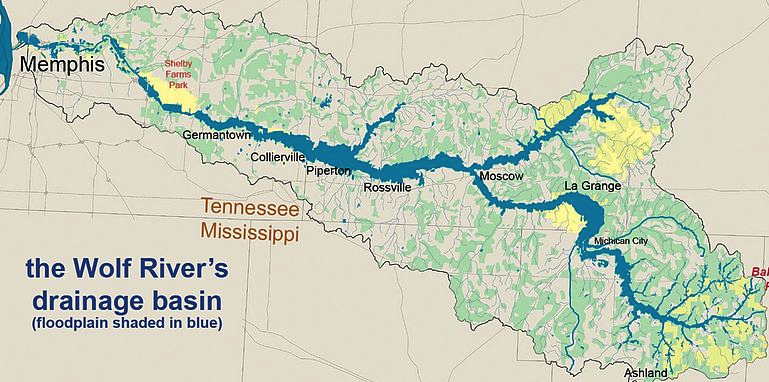
\includegraphics[width=0.5\textwidth]{\chp7@path/7-5_anova/figures/aldrin/wolf}
\end{center}

{\small
\begin{itemize}

\item  The Wolf River in Tennessee flows past an abandoned site once used by the pesticide industry for dumping wastes, including chlordane (pesticide), aldrin, and dieldrin (both insecticides).

\pause

\item These highly toxic organic compounds can cause various cancers and birth defects.

\pause

\item The standard methods to test whether these substances are present in a river is to take samples at six-tenths depth. 

\pause

\item But since these compounds are denser than water and their molecules tend to stick to particles of sediment, they are more likely to be found in higher concentrations near the bottom than near mid-depth.

\end{itemize}
}

\end{frame}

%%%%%%%%%%%%%%%%%%%%%%%%%%%%%%%%%%%

\begin{frame}
\frametitle{Data}

Aldrin concentration (nanograms per liter) at three levels of depth. \\

\begin{center}
\begin{tabular}{r | c | c}
\hline
 	& aldrin 					& depth \\ 
\hline
1 	& \textcolor{darkGray}{3.80} 	& \textcolor{darkGray}{bottom}  \\ 
2 	& \textcolor{darkGray}{4.80} 	& \textcolor{darkGray}{bottom}  \\ 
...	&						& \\
10	& \textcolor{darkGray}{8.80} 	& \textcolor{darkGray}{bottom} \\
11	& \textcolor{blue}{3.20} 		& \textcolor{blue}{middepth}  \\
12	& \textcolor{blue}{3.80} 		& \textcolor{blue}{middepth} \\
...	&						& \\
20 	& \textcolor{blue}{6.60} 		& \textcolor{blue}{middepth} \\
21	& \textcolor{oiB}{3.10} 		& \textcolor{oiB}{surface} \\
22	& \textcolor{oiB}{3.60} 		& \textcolor{oiB}{surface} \\
...	&						& \\
30 	& \textcolor{oiB}{5.20} 		& \textcolor{oiB}{surface} \\  
\hline
\end{tabular}
\end{center}

\end{frame}

%%%%%%%%%%%%%%%%%%%%%%%%%%%%%%%%%%%

\begin{frame}
\frametitle{Exploratory analysis}

Aldrin concentration (nanograms per liter) at three levels of depth. \\

\begin{center}
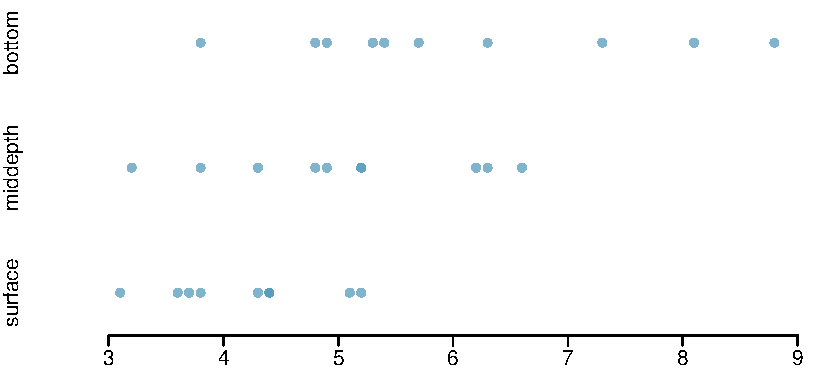
\includegraphics[width=0.75\textwidth]{\chp7@path/7-5_anova/figures/aldrin/dotplot}
\end{center}

\begin{center}
\begin{tabular}{l | c c c}
		& n	& mean	& sd		\\
\hline
bottom	& 10	& 6.04	& 1.58 \\
middepth& 10	& 5.05	& 1.10 \\
surface	& 10	& 4.20	& 0.66 \\
\hline
overall	& 30	& 5.1	0	& 1.37
\end{tabular}
\end{center}

\end{frame}

%%%%%%%%%%%%%%%%%%%%%%%%%%%%%%%%%%%

\begin{frame}
\frametitle{Research question}

\dq{Is there a difference between the mean aldrin concentrations among the three levels?}

\vspace{0.5cm}

\pause

\begin{itemize}

\item To compare means of 2 groups we use a Z or a T statistic.

\pause

\item To compare means of 3+ groups we use a new test called \hl{ANOVA} and a new statistic called \hl{F}.

\end{itemize}

\end{frame}

%%%%%%%%%%%%%%%%%%%%%%%%%%%%%%%%%%%

\begin{frame}
\frametitle{ANOVA}

ANOVA is used to assess whether the mean of the outcome variable is different for different levels of a categorical variable.

\pause

\begin{itemize}
\item[] \mathhl{H_0:} The mean outcome is the same across all categories, 
\[\mu_1 = \mu_2 = \cdots = \mu_k, \]
where $\mu_i$ represents the mean of the outcome for observations in category $i$.
\item[]
\item[] \mathhl{H_A:} At least one mean is different than others.
\end{itemize}

\end{frame}

%%%%%%%%%%%%%%%%%%%%%%%%%%%%%%%%%%%

\begin{frame}
\frametitle{Conditions}

\begin{enumerate}

\item The observations should be independent within and between groups

\begin{itemize}
\item If the data are a simple random sample from less than 10\% of the population, this condition is satisfied.
\item Carefully consider whether the data may be independent (e.g. no pairing). 
\item Always important, but sometimes difficult to check.
\end{itemize}

\pause

\item The observations within each group should be nearly normal.

\begin{itemize}
\item Especially important when the sample sizes are small.
\end{itemize}

\dq{How do we check for normality?}

\pause

\item The variability across the groups should be about equal.

\begin{itemize}
\item Especially important when the sample sizes differ between groups.
\end{itemize}

\dq{How can we check this condition?}

\end{enumerate}

\end{frame}

%%%%%%%%%%%%%%%%%%%%%%%%%%%%%%%%%%%

\begin{frame}
\frametitle{$z$/$t$ test vs. ANOVA - Purpose}

\twocol{0.5}{0.5}
{
\[ \hl{$z$/$t$ test} \]
Compare means from \hl{two} groups to see whether they are so far apart that the observed difference cannot reasonably be attributed to sampling variability.
\[ H_0: \mu_1 = \mu_2 \]
}
{
\[ \hl{ANOVA} \]
Compare the means from \hl{two or more} groups to see whether they are so far apart that the observed differences cannot all reasonably be attributed to sampling variability.
\[ H_0: \mu_1 = \mu_2 = \cdots = \mu_k \]
}

\end{frame}

%%%%%%%%%%%%%%%%%%%%%%%%%%%%%%%%%%%

\begin{frame}
\frametitle{$z$/$t$ test vs. ANOVA - Method}

\twocol{0.5}{0.5}
{
\[ \hl{$z$/$t$ test} \]
Compute a test statistic (a ratio).
\[ z / t = \frac{(\bar{x}_1 - \bar{x}_2) - (\mu_1 - \mu_2)}{SE(\bar{x}_1 - \bar{x}_2)} \]
}
{
\[ \hl{ANOVA} \]
Compute a test statistic (a ratio).
\[ F = \frac{\text{variability bet. groups}}{\text{variability w/in groups}} \]
}

\vspace{1cm}

\pause

\begin{itemize}

\item Large test statistics lead to small p-values. 

\item If the p-value is small enough $H_0$ is rejected, we conclude that the population means are not equal.

\end{itemize}

\end{frame}

%%%%%%%%%%%%%%%%%%%%%%%%%%%%%%%%%%%

\begin{frame}
\frametitle{$z$/$t$ test vs. ANOVA}

\begin{itemize}

\item With only two groups t-test and ANOVA are equivalent, but only if we use a pooled standard variance in the denominator of the test statistic.

\pause

\item With more than two groups, ANOVA compares the sample means to an overall \hl{grand mean}.

\end{itemize}

\end{frame}

%%%%%%%%%%%%%%%%%%%%%%%%%%%%%%%%%%%

\section{Edfinity Quiz: Setting the Hypotheses}

%%%%%%%%%%%%%%%%%%%%%%%%%%%%%%%%%%%

\begin{frame}
\frametitle{Hypotheses}

\pq{What are the correct hypotheses for testing for a difference between the mean aldrin concentrations among the three levels?}

\begin{enumerate}[(a)]
\item $H_0: \mu_B = \mu_M = \mu_S$ \\
$H_A: \mu_B \ne \mu_M \ne \mu_S$ \\
\item $H_0: \mu_B \ne \mu_ M \ne \mu_S$ \\
$H_A: \mu_B = \mu_M = \mu_S$ \\
\solnMult{$H_0: \mu_B = \mu_M = \mu_S$ \\
$H_A:$ At least one mean is different.}
\item $H_0: \mu_B = \mu_M = \mu_S = 0$ \\
$H_A:$ At least one mean is different.
\item $H_0: \mu_B = \mu_M = \mu_S$ \\
$H_A: \mu_B > \mu_M > \mu_S$ \\
\end{enumerate}

\end{frame}

%%%%%%%%%%%%%%%%%%%%%%%%%%%%%%%%%%%

\subsection{ANOVA and the F test}

%%%%%%%%%%%%%%%%%%%%%%%%%%%%%%%%%%%

\begin{frame}
\frametitle{Test statistic}

\dq{Does there appear to be a lot of variability within groups? How about between groups?}

\[ F = \frac{\text{variability bet. groups}}{\text{variability w/in groups}}  \]

\begin{center}
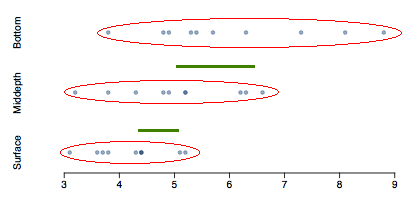
\includegraphics[width=0.75\textwidth]{\chp7@path/7-5_anova/figures/aldrin/dotplot_var}
\end{center}

\end{frame}

%%%%%%%%%%%%%%%%%%%%%%%%%%%%%%%%%%%

%\begin{frame}
%\frametitle{Test statistic (cont.)}
%
%\[ F = \frac{\text{variability bet. groups}}{\text{variability w/in groups}} = \frac{\hl{MSG}}{\hl{MSE}}  \]
%
%\begin{itemize}
%
%\item \hl{MSG} is mean square between groups
%\[ df_G = k - 1 \]
%where $k$ is number of groups
%
%\item \hl{MSE} is mean square error - variability in residuals
%\[ df_E = n - k \]
%where $n$ is number of observations.
%
%\end{itemize}
%
%\end{frame}
%
%%%%%%%%%%%%%%%%%%%%%%%%%%%%%%%%%%%%

\begin{frame}
\frametitle{$F$ distribution and p-value}

\[ F =  \frac{\text{variability bet. groups}}{\text{variability w/in groups}} \]

\vspace{-1cm}

\begin{center}
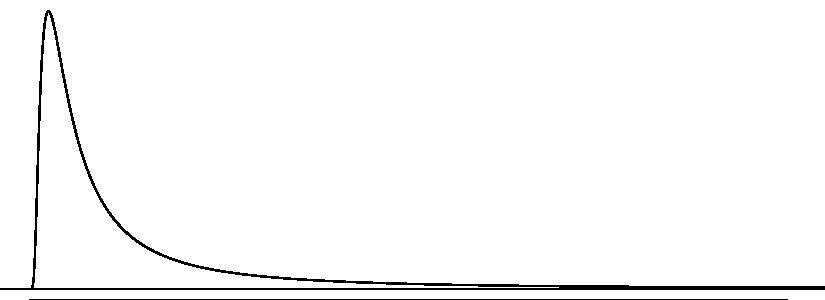
\includegraphics[width=0.75\textwidth]{\chp7@path/7-5_anova/figures/fdist/fdist}
\end{center}

\begin{itemize}

\item In order to be able to reject $H_0$, we need a small p-value, which requires a large F statistic.

\item In order to obtain a large F statistic, variability between sample means needs to be greater than variability within sample means.

\end{itemize}

\end{frame}

%%%%%%%%%%%%%%%%%%%%%%%%%%%%%%%%%%%

\subsection{ANOVA output, deconstructed}

%%%%%%%%%%%%%%%%%%%%%%%%%%%%%%%%%%%

\begin{frame}
\frametitle{}

\vspace{-0.5cm}

{\footnotesize
\begin{center}
\begin{tabular}{ll >{\columncolor[gray]{.6}[.5\tabcolsep]}rrrrr}
\hline
 			& 			& Df 	& Sum Sq	& Mean Sq 	& F value 	& Pr($>$F) \\ 
\hline
(\hl{G}roup) 	& depth 		& 2 	& 16.96 	& 8.48 		& 6.13 	& 0.0063 \\ 
(\hl{E}rror) 	& Residuals 	& 27 	& 37.33 	& 1.38 		&  		&  \\ 
\hline
	 		& \hl{T}otal	& 29	& 54.29 \\
\end{tabular}
\end{center}
}

\formula{Degrees of freedom associated with ANOVA}
{
\begin{itemize}
\item groups: $df_G = k - 1$, where $k$ is the number of groups
\item total: $df_T = n - 1$, where $n$ is the total sample size
\item error: $df_E = df_T - df_G$
\end{itemize}
}

\pause

\begin{itemize}

\item $df_G = k - 1 = 3 - 1 = 2$ \\ 

\pause

\item $df_T = n - 1 = 30 - 1 = 29$

\pause

\item $df_E = 29 - 2 = 27$ \\

\end{itemize}

\end{frame}

%%%%%%%%%%%%%%%%%%%%%%%%%%%%%%%%%%%

\section{R Demonstration: Group computations, statistics}
% Thinking of the R Demo replacing the slides on these items, but unsure where to split for the next lecture. 
% Trying ending on the F statistic here and continuing next time with the p-value.

%%%%%%%%%%%%%%%%%%%%%%%%%%%%%%%%%%%


\begin{frame}
\frametitle{}

\vspace{-0.25cm}

{\footnotesize
\begin{center}
\begin{tabular}{ll r>{\columncolor[gray]{.6}[.5\tabcolsep]}rrrr}
\hline
 			& 			& Df 	& Sum Sq	& Mean Sq 	& F value 	& Pr($>$F) \\ 
\hline
(\hl{G}roup) 	& depth 		& 2 	& \orange{16.96} 	& 8.48 		& 6.13 	& 0.0063 \\ 
(\hl{E}rror) 	& Residuals 	& 27 	& 37.33 	& 1.38 		&  		&  \\ 
\hline
	 		& \hl{T}otal	& 29	& 54.29 \\
\end{tabular}
\end{center}
}

\formula{Sum of squares between groups, SSG}
{
Measures the variability between groups 
\vspace{-0.25cm}
\[ SSG = \sum_{i = 1}^{k} n_i (\bar{x}_i - \bar{x})^2 \]
where $n_i$ is each group size, $\bar{x}_i$ is the average for each group, $\bar{x}$ is the overall (grand) mean.
}

\pause

\vspace{-0.5cm}

\twocol{0.4}{0.5}
{
{\small
\begin{center}
\begin{tabular}{l | c c }
		& n	& mean		\\
\hline
bottom	& 10	& 6.04	 \\
middepth& 10	& 5.05	 \\
surface	& 10	& 4.2	 \\
\hline
overall	& 30	& 5.1	
\end{tabular}
\end{center}
}
}
{
\pause
\begin{eqnarray*}
SSG &=& \pr{ 10 \times (6.04 - 5.1)^2 } \\
\pause
&+& \pr{ 10 \times (5.05 - 5.1)^2 } \\
\pause
&+& \pr{ 10 \times (4.2 - 5.1)^2 } \\
\pause
&=& 16.96 \\
\end{eqnarray*}
}

\end{frame}

%%%%%%%%%%%%%%%%%%%%%%%%%%%%%%%%%%%

\begin{frame}
\frametitle{}

\vspace{-0.25cm}

{\footnotesize
\begin{center}
\begin{tabular}{ll r>{\columncolor[gray]{.6}[.5\tabcolsep]}rrrr}
\hline
 			& 			& Df 	& Sum Sq	& Mean Sq 	& F value 	& Pr($>$F) \\ 
\hline
(\hl{G}roup) 	& depth 		& 2 	& 16.96	& 8.48 		& 6.13 	& 0.0063 \\ 
(\hl{E}rror) 	& Residuals 	& 27 	& 37.33 	& 1.38 		&  		&  \\ 
\hline
	 		& \hl{T}otal	& 29	& \orange{54.29} \\
\end{tabular}
\end{center}
}

\formula{Sum of squares total, SST}
{
Measures the variability between groups 
\vspace{-0.25cm}
\[ SST = \sum_{i = 1}^{n} (x_i - \bar{x})^2 \]
where $x_i$ represent each observation in the dataset.
}

\pause

\vspace{-0.75cm}

\begin{eqnarray*}
SST &=& (3.8 - 5.1)^2 + (4.8 - 5.1)^2 + (4.9 - 5.1)^2 + \cdots + (5.2 - 5.1)^2 \\
\pause
&=& (-1.3)^2 + (-0.3)^2 + (-0.2)^2 + \cdots + (0.1)^2 \\
\pause
&=& 1.69 + 0.09 + 0.04 + \cdots + 0.01 \\
\pause
&=& 54.29
\end{eqnarray*}

\end{frame}

%%%%%%%%%%%%%%%%%%%%%%%%%%%%%%%%%%%

\begin{frame}
\frametitle{}

\vspace{-0.25cm}

{\footnotesize
\begin{center}
\begin{tabular}{ll r>{\columncolor[gray]{.6}[.5\tabcolsep]}rrrr}
\hline
 			& 			& Df 	& Sum Sq	& Mean Sq 	& F value 	& Pr($>$F) \\ 
\hline
(\hl{G}roup) 	& depth 		& 2 	& 16.96	& 8.48 		& 6.13 	& 0.0063 \\ 
(\hl{E}rror) 	& Residuals 	& 27 	& \orange{37.33} 	& 1.38 		&  		&  \\ 
\hline
	 		& \hl{T}otal	& 29	& 54.29 \\
\end{tabular}
\end{center}
}

\formula{Sum of squares error, SSE}
{
Measures the variability within groups:
\[ SSE = SST - SSG \]
}

\pause

\[ SSE =  54.29 - 16.96 =  37.33 \]

\end{frame}

%%%%%%%%%%%%%%%%%%%%%%%%%%%%%%%%%%%

\begin{frame}
\frametitle{}

\vspace{-0.25cm}

{\footnotesize
\begin{center}
\begin{tabular}{ll rr>{\columncolor[gray]{.6}[.5\tabcolsep]}rrr}
\hline
 			& 			& Df 	& Sum Sq	& Mean Sq 	& F value 	& Pr($>$F) \\ 
\hline
(\hl{G}roup) 	& depth 		& 2 	& 16.96	& \orange{8.48} 		& 6.13 	& 0.0063 \\ 
(\hl{E}rror) 	& Residuals 	& 27 	& 37.33 	& \orange{1.38} 		&  		&  \\ 
\hline
	 		& \hl{T}otal	& 29	& 54.29 \\
\end{tabular}
\end{center}
}

\formula{Mean square error}
{
Mean square error is calculated as sum of squares divided by the degrees of freedom.
}

\pause

\begin{eqnarray*}
MSG &=& 16.96 / 2 = 8.48 \\
\pause
MSE &=& 37.33 / 27 = 1.38
\end{eqnarray*}

\end{frame}

%%%%%%%%%%%%%%%%%%%%%%%%%%%%%%%%%%%

\begin{frame}
\frametitle{}

\vspace{-0.25cm}

{\footnotesize
\begin{center}
\begin{tabular}{ll rrr>{\columncolor[gray]{.6}[.5\tabcolsep]}rr}
\hline
 			& 			& Df 	& Sum Sq	& Mean Sq 	& F value 	& Pr($>$F) \\ 
\hline
(\hl{G}roup) 	& depth 		& 2 	& 16.96	& 8.48 		& \orange{6.14} 	& 0.0063 \\ 
(\hl{E}rror) 	& Residuals 	& 27 	& 37.33 	& 1.38 		&  		&  \\ 
\hline
	 		& \hl{T}otal	& 29	& 54.29 \\
\end{tabular}
\end{center}
}

\formula{Test statistic, F value}
{
As we discussed before, the F statistic is the ratio of the between group and within group variability.
\[ F = \frac{MSG}{MSE} \]
}

\pause

\[ F = \frac{8.48}{1.38} = 6.14 \]

\end{frame}

%%%%%%%%%%%%%%%%%%%%%%%%%%%%%%%%%%%%

%%%%%%%%%%%%%%%%%%%%%%%%%%%%%%%%%%%%
% End document
%%%%%%%%%%%%%%%%%%%%%%%%%%%%%%%%%%%%

\end{document}